
\documentclass{article}

\usepackage{times}
\usepackage{epsfig}
\usepackage{graphicx}
\usepackage{amsmath}
\usepackage{amssymb}

% Include other packages here, before hyperref.

% If you comment hyperref and then uncomment it, you should delete
% egpaper.aux before re-running latex.  (Or just hit 'q' on the first latex
% run, let it finish, and you should be clear).
\usepackage[pagebackref=true,breaklinks=true,colorlinks,bookmarks=false]{hyperref}


% my own packages
\usepackage{xcolor}


\newcommand{\bX}{\mathbf{X}}
\newcommand{\bx}{\mathbf{x}}
\newcommand{\mb}[1]{\mathbf{#1}}
\newcommand{\mc}[1]{\mathcal{#1}}
\newcommand{\mbh}[1]{\hat{\mathbf{#1}}}


\newcommand{\bC}{\mathbf{C}}
\newcommand{\bn}{\mathbf{n}}
\newcommand{\bh}{\mathbf{h}}
\newcommand{\bD}{\mathbf{D}}
\newcommand{\bT}{\mathbf{T}}


%\setcounter{page}{4321} % For final version only


\begin{document}

%%%%%%%%% TITLE
\title{Least Squares}

\author{David Ivan \\
{\tt\small avandavad@gmail.com}
% For a paper whose authors are all at the same institution,
% omit the following lines up until the closing ``}''.
% Additional authors and addresses can be added with ``\and'',
% just like the second author.
% To save space, use either the email address or home page, not both
}

\maketitle


\section{Direct measurements}

\subsection{Theory}

We want to estimate $\bar{x}$. The measurements are $y_i$ ($i \in \{1,2,\dots,k\}$), with uncertainties $R_i$. So $y_i$ is normally distributed with mean $\bar{x}$, covariance $R_i$.

\begin{equation}
\begin{split}
    y_i &= \bar{x} + v_i \\
    &v_i \sim N(0, R_i)
\end{split}
\end{equation}

$v_i$ are the error vectors. The energy term to minimize:

\begin{equation}
    E(x) = \sum_{i=1}^{k} (x - y_i)^T R^{-1}_i (x - y_i)
\end{equation}

Let's calculate the derivative of $E(x)$ w.r.t. $x$:

\begin{equation}
    \frac{\partial E}{\partial x} = \sum_{i=1}^{k} 2 (x - y_i)^T R^{-1}_i
\end{equation}

Setting the derivative to zero, and solving for $x$:

\begin{equation}
    \boxed{\hat{x} = \left( \sum_{i=1}^{k} R^{-1}_i \right)^{-1} \cdot \sum_{i=1}^{k} R^{-1}_i y_i}
\end{equation}

The variance of the estimation (assuming that the measurements are independent) can be easily calculated, the result is:

\begin{equation}
    \boxed{\text{Var}(\hat{x}) = \left( \sum_{i=1}^{k} R^{-1}_i \right)^{-1}}
\end{equation}

\begin{equation}
    \hat{x}
\end{equation}

\subsection{Example}

Figure \ref{fig:1} shows an example where we have 3 measurements for estimating $\bar{x}$.

\begin{figure}
    \centering
    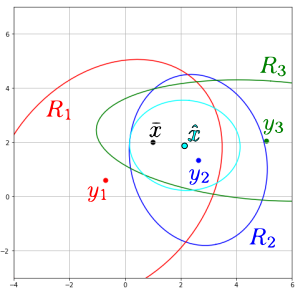
\includegraphics[scale=0.6]{pic1.png}
    \caption{Example. We have 3 measurements $y_1$, $y_2$ and $y_3$ with the corresponding covariance matrices $R_i$. $\hat{x}$ is the maximum likelihood solution. Note that the uncertainty of $\hat{x}$ is less than any of the measurements.}
    \label{fig:1}
\end{figure}

\end{document}